
  
\noindent {\color{special}{\Large \bf Para o professor}}
\vspace{.5cm}
  
  Reconhecer quando duas frações são iguais, saber gerar frações iguais a uma 
dada fração e obter duas frações de mesmo denominador que são iguais a duas 
frações quaisquer dadas são habilidades fundamentais que permitem resolver 
vários problemas no estudo de frações.  Por exemplo, com essas habilidades, é 
possível criar procedimentos que permitem comparar duas frações com 
denominadores diferentes e obter uma fração que está entre duas frações 
diferentes (propriedade de densidade das frações). São esses tópicos que compõem 
a presente lição.  
  
  O processo de comparação de frações com denominadores distintos é apresentado 
como motivação, em uma situação problema, em formato de história em quadrinho, 
logo no início da lição. Contudo sua solução é retomada na seção   {\it 
Organizando as ideias}  , após a apresentação das oito primeiras atividades que 
compõem a seção   {\it Explorando o Assunto}  . Estas atividades iniciais 
abordam basicamente a igualdade de frações. Todas elas encontram-se organizadas 
em ordem crescente de dificuldade. O conceito de igualdade é abordado 
utilizando-se representações equivalentes em modelos de área retangulares 
(atividades 2  , 3   e 6), ou em modelos de área circulares (atividade 5) ou na 
reta numérica (atividade 8). A inclusão de modelos diferentes é proposital pois, 
com isso, o aluno tem a oportunidade de perceber as mesmas propriedades em 
contextos diferentes aumentando assim o seu arsenal de modelos que ele pode 
lançar mão ao justificar uma resposta ou estudar uma situação.  
  
  Cabe destacar aqui um detalhe sutil, mas que permeia toda a lição: trata-se do 
uso das expressões   ``frações equivalentes''   e   ``frações iguais''  . Nesta 
lição, a expressão   ``frações equivalentes''   é usada se as frações em questão 
estiverem associadas a divisões de algum objeto físico (bolo, torta, pizza, 
chocolate, etc.), de forma a poder exprimir o fato de que processos de partições 
diferentes podem gerar quantidades iguais. Por exemplo, o processo de dividir um 
bolo ao meio e pegar uma das partes é diferente daquele em que o bolo é dividido 
quatro partes iguais e se toma duas dessas partes. No entanto, em termos de 
quantidades, tem-se, em ambos os casos a metade do bolo. Já a expressão   
``frações iguais''   será usada se as frações se referem a números, sem um 
contexto específico. Por exemplo,   $\frac{2}{4}$   é a única fração de 
denominador 4 que é igual a   $\frac{1}{2}$. No entanto, cabe ressaltar que não 
se espera que os alunos sejam capazes de registrar este tipo de diferença. 
Assim, recomenda-se que os usos, por parte dos alunos, das expressões frações 
equivalentes e frações iguais nos contextos destacados sejam considerados 
igualmente válidos e indistinguíveis.  
  
  As sistematizações dos procedimentos de   {\bf comparação}   (atividades 12  , 
13  , 14  , 15   e 18  ) e do conceito de   {\bf igualdade}   de frações 
(atividades 9  , 10  , 11  , 16  , 17  , 19   e 20  ) são então realizadas na 
seção   {\it Mão na Massa}  . O processo de determinação da fração irredutível 
igual à fração dada é, por exemplo, trabalhado nas atividades 16   e 17  . Uma 
condição suficiente para verificação da igualdade de frações é apresentada na 
atividade 19  . O jogo   {\bf Trilha dos doze avos}   (\emph{atividade 20}  ) é 
uma boa estratégia para que se possa consolidar de forma prazerosa a igualdade 
de frações.   
  
  Na parte final da lição, na seção   {\it Quebrando a Cuca}  , apresentam-se 
atividades que sugerem uma avaliação crítica pelos alunos de afirmações que 
generalizam situações de igualdade e de comparação entre frações. Cabe destacar 
que todas as atividades desta última seção, em especial, deverão ser conduzidas 
sem pressa, por meio de debates intensos entre os alunos para que os argumentos 
equivocados apareçam e possam ser descontruídos por eles próprios.  
  
  Tanto a comparação de frações arbitrárias como o estudo da propriedade de 
densidade apresenta como procedimento base a procura por representações 
equivalentes de frações dadas. Nesse sentido, destaca-se a técnica utilizada nas 
atividades 23   e 24   para determinar uma fração intermediária entre duas 
frações arbitrárias dadas. A técnica, que consiste simplesmente em procurar 
frações intermediárias por meio de representações equivalentes das frações dadas 
com denominadores iguais e suficientemente grandes, além de original, supera o 
procedimento usual (que utiliza a adição de frações e a divisão de uma fração 
por um número natural), por sua simplicidade e naturalidade. Este resultado, 
conhecido no âmbito pedagógico como   ``propriedade de densidade dos números 
racionais''  , não se verifica para os conjuntos de números naturais e de 
números inteiros, e é, sem dúvida, um dos fatos mais notáveis na extensão que se 
faz do conjunto dos números inteiros para o conjunto dos números racionais.  É a 
responsável, por exemplo, pelo fato de um número racional não ter elemento 
sucessor.   
  
  Cabe lembrar que as habilidades desenvolvidas nessa lição são fundamentais 
para as lições seguintes que tratam das operações com frações.  
  \vspace{.15cm}

\noindent OBJETIVOS ESPECÍFICOS DA LIÇÃO 4:
\vspace{.15cm}

\noindent O aluno deve ser capaz de:  
  
\begin{itemize} %d
    \item       Reconhecer a igualdade de frações, seja por representações 
geométricas ou por representações numéricas equivalentes;
    \item       Determinar frações equivalentes por subdivisões de uma fração 
dada;
    \item       Identificar a representação de frações iguais (equivalentes) na 
reta numérica;
    \item       Reconhecer a igualdade de duas frações por processo matemático 
suficiente (se       $a \times d = b \times c$, então       $\frac{a}{b} = 
\frac{c}{d}$);
    \item       Simplificar frações;
    \item       Comparar duas ou mais frações com denominadores diferentes;
    \item       Reconhecer a fração (o número racional não negativo) como uma 
classe de equivalência;
    \item       Determinar, dada uma fração arbitrária, sua fração irredutível;
    \item       Reconhecer a propriedade de densidade do conjunto de frações 
(números racionais não negativos);
    \item       Determinar uma fração, entre duas frações dadas, com base em 
representações equivalentes dessas frações com denominadores suficientemente 
grandes.
\end{itemize} %d


\begin{multicols}{2}



\subsection{Atividade 1}

  \noindent {\bf Objetivos específicos: Levar o aluno a }  
\begin{itemize} %s
    \item       Reconhecer que as frações       $\frac{1}{2}$       e       
$\frac{2}{4}$       são iguais a partir da observação das representações destas 
frações em modelos de área retangulares.
    \item       Reconhecer que, em uma equipartição de uma região retangular, só 
é possível escolher uma quantidade de partes que corresponda à metade desta 
região se a quantidade total de partes for um número par.
    \item       É importante, ao final da atividade, observar para os alunos que 
uma mesma parte do retângulo (metade do retângulo) está sendo descrita por 
frações com numeradores e denominadores diferentes (isto é, por frações 
equivalentes) mas que, não obstante, por expressarem uma mesma quantidade, estas 
frações são iguais. Assim,       $\frac{1}{2}$,       $\frac{2}{4}$,       
$\frac{4}{8}$, etc. são respostas válidas para o item b) desta atividade.
\end{itemize} %s
  
  
  \noindent {\bf Recomendações e sugestões para o desenvolvimento da atividade:} 
 
  
\begin{itemize} %s
    \item       Recomenda-se que, nesta atividade, os alunos trabalhem 
individualmente ou em duplas. No entanto, é fundamental que os alunos sejam 
estimulados a explicar o raciocínio realizado.
    \item       Reforce para seus alunos que o item b) deve ser respondido com a 
partição apresentada, isto é, sem gerar novas partições.
    \item       Observe que o item c) pode ser respondido apenas pela fração     
  $\frac{1}{2}$. No entanto, é importante estimular os alunos a pereceberem que 
a metade do sanduíche pode ser obtida por       $\frac{2}{4}$       do 
sanduíche. 
\end{itemize} %s
  
  
  Classificações:  
\begin{itemize} %s
    \item       Heid et al.: Conceito: identificar e descrever
    \item       Nicely, Jr.: Nível 1: reconhecer
    \item       UERJ: Observar: identificar e reconhecer
\end{itemize} %s
  

\begin{resposta*}{Atividade 1}  
\begin{enumerate} [\quad a)] %s
    \item       Em a):       $\frac{1}{2}$. Em b):       $\frac{1}{3}$. Em c):   
    $\frac{1}{4}$. Em d):       $\frac{1}{4}$.
    \item       É possível comer metade do sanduíche apenas nas repartições a), 
c) e d) pois, para elas, a quantidade de partes iguais em que o sanduíche foi 
dividido é um número par.
    \item       Em a):       $\frac{1}{2}$. Em c):       $\frac{2}{4}$. Em d):   
    $\frac{2}{4}$.
\end{enumerate} %s
  
\end{resposta*}





\subsection{Atividade 2}

 \noindent {\bf Objetivo específico: Levar o aluno a}  
\begin{itemize} %s
    \item       Reconhecer que as frações       $\frac{3}{10}$,       
$\frac{6}{20}$,       $\ldots$,       $\frac{3 \times m}{10 \times m}$       são 
iguais a partir da observação das representações destas frações em modelos de 
área retangulares e dobraduras. 
\end{itemize} %s
  
  
  \noindent {\bf Recomendações e sugestões para o desenvolvimento da atividade:} 
 
\begin{itemize} %s
    \item       Recomenda-se que a atividade seja desenvolvida em grupos de 3 a 
5 alunos e que, neste caso, cada grupo receba uma quantidade suficiente de 
cópias das             folhas para reprodução      . Podem ser necessárias mais 
do que uma dessas folhas por aluno. Uma vez que a folha já tenha sido dobrada 
para a realização de um dos itens, a marca deixada pode atrapalhar a realização 
do item seguinte. 
    \item       É importante deixar claro para os alunos que, para decidir sobre 
a quantidade de retângulos pintados e a quantidade total de retângulos, se devem 
considerar as divisões feitas pelos vincos das dobras. Neste sentido, você pode, 
junto com a turma, a título de exemplo e de orientação, preencher a segunda 
linha da tabela, deixando as demais para sejam preenchidas pelos grupos.
    \item       É importante, ao final da atividade, observar para os alunos que 
uma mesma parte do retângulo (a área da região pintada de amarelo) está sendo 
descrita por frações com numeradores e denominadores diferentes (isto é, por 
frações equivalentes), mas que, não obstante, por expressarem uma mesma 
quantidade, estas frações são iguais. 
\end{itemize} %s
  
  
  Classificações:  
\begin{itemize} %s
    \item       Heid et al.: Conceito: identificar e descrever
    \item       Nicely, Jr.: Nível 1: reconhecer
    \item       UERJ: Observar: identificar e reconhecer
\end{itemize} %s
  
  \end{multicols}
  \pagebreak
  
\begin{resposta*}{Atividade 2}
  
\noindent 
\begin{tabular}{|m{.3\textwidth}|m{.16\textwidth}|m{.16\textwidth}|m{.21\textwidth}|}
    \hline
      Como dobrar  &  quantidade de retângulos pintados  & Quantidade total de retângulos  &  Fração do retângulo do encarte que está pintada  \\
    \hline \hline   
       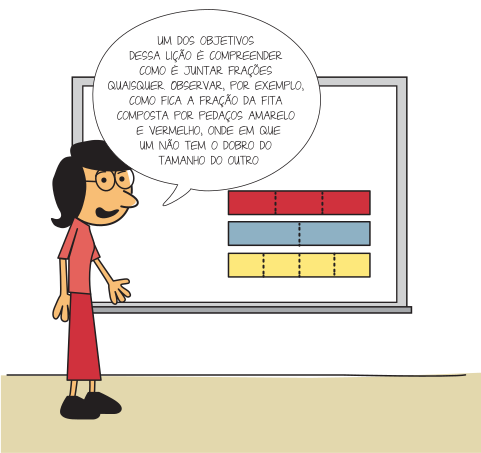
\includegraphics[width=110pt, 
keepaspectratio]{../../livro/media/cap4/secoes/PNGs/ativ2_fig01.png} &  3 &  10 &  
$\frac{3}{10}$ \\
      \hline 
       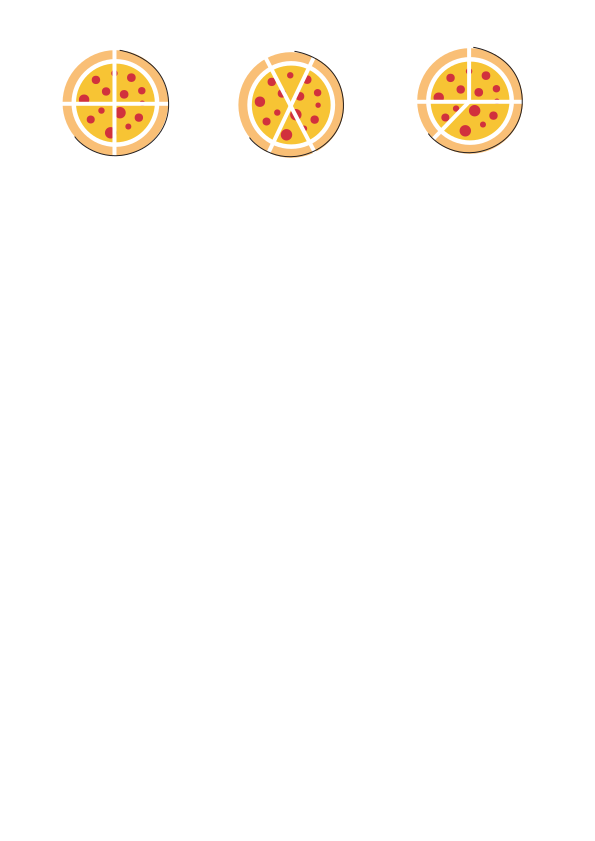
\includegraphics[width=110pt, 
keepaspectratio]{../../livro/media/cap4/secoes/PNGs/ativ2_fig02.png} &  6 &  20 &  
$\frac{6}{20}$ \\
      \hline 
       
\includegraphics[width=110pt, 
keepaspectratio]{../../livro/media/cap4/secoes/PNGs/ativ2_fig03.png} &  9 &  30 &  
$\frac{9}{30}$ \\
      \hline 
       \includegraphics[width=110pt, 
keepaspectratio]{../../livro/media/cap4/secoes/PNGs/ativ2_fig04.png} &  12 &  40 &  
$\frac{12}{40}$ \\
      \hline 
      \includegraphics[width=110pt, keepaspectratio]{../../livro/media/cap4/secoes/PNGs/ativ2_fig05.png}&  18 &  60 &  $\frac{18}{60}$ \\
      \hline 
      \includegraphics[width=110pt, keepaspectratio]{../../livro/media/cap4/secoes/PNGs/ativ2_fig06.png}&  24 &  80 &  $\frac{24}{80}$ \\
      \hline 
    \end{tabular}
  
\end{resposta*}

\Bg

\begin{multicols}{2}
\subsection{Atividade 3}


 \noindent {\bf Objetivo específico: Levar o aluno a}  
\begin{itemize} %s
    \item       Reconhecer que as frações       $\frac{3}{4}$       e       
$\frac{12 \times 3}{12 \times 4}$       são iguais a partir da observação das 
representações destas frações em modelos de área sem a contagem um a um das 
partes que compõem as subdivisões destas representações.
\end{itemize} %s
  
  
  \noindent {\bf Recomendações e sugestões para o desenvolvimento da atividade:} 
 
\begin{itemize} %s
    \item       Recomenda-se que, nesta atividade, os alunos trabalhem 
individualmente ou em duplas. No entanto, é fundamental que os alunos sejam 
estimulados a explicar o raciocínio realizado.
    \item       O propósito de encobrir as divisões do retângulo é para evitar 
que os alunos façam a contagem das partes uma a uma e que, assim, sejam 
estimulados a perceber a estrutura multiplicativa       $12 \times 3$       e    
   $12 \times 4$       na divisão do retângulo.
    \item       É importante, ao final da atividade, observar para os alunos que 
uma mesma parte do retângulo (a área da região pintada de azul) está sendo 
descrita por frações com numeradores e denominadores diferentes (isto é, por 
frações equivalentes), mas que, não obstante, por expressarem uma mesma 
quantidade, estas frações são iguais. 
\end{itemize} %s
  
  
  Classificações:  
\begin{itemize} %s
    \item       Heid et al.: Produto: prever
    \item       Nicely, Jr.: Nível 1: reconhecer
    \item       UERJ: Interpretar: compor e decompor
\end{itemize} %s
  
\begin{resposta*}{Atividade 3}  
\begin{enumerate} [\quad a)] %s
    \item             $\frac{3}{4}$.
    \item       Com a nova divisão, o retângulo fica dividido em       $12 
\times 4 = 48$       partes, das quais       $12 \times 3 = 36$       está 
pintada de azul. Assim, a fração do retângulo que está pintada de azul é igual a 
      $\frac{12 \times 3}{12 \times 4} = \frac{36}{48}$.
\end{enumerate} %s
  
\end{resposta*}



\subsection{Atividade 4}

  \noindent {\bf Objetivos específicos: Levar o aluno a }  
\begin{itemize} %s
    \item       Comparar frações, em que os denominadores são múltiplos, a 
partir de modelos contínuos.
    \item       Introduzir a discusão sobre frações equivalentes    
\end{itemize} %s
  
      
  \noindent {\bf Recomendações e sugestões para o desenvolvimento da atividade:} 
 
\begin{enumerate} [\quad a)] %s
    \item       Recomenda-se que, nesta atividade, os alunos trabalhem 
individualmente ou em duplas. No entanto, é fundamental que os alunos sejam 
estimulados a explicar o raciocínio realizado.
    \item       Para amparar a reflexão dos alunos, recomenda-se que sejam 
feitas cópias das             folhas para reprodução disponíveis no final do 
livro      .
    \item       Não se recomenda que a nomenclatura       ``frações 
equivalentes''       seja introduzida em sala de aula. Por exemplo, pode-se 
falar apenas que as frações 1/2 e 2/4 representam a mesma quantidade, e por isso 
têm a mesma representação na reta numérica.
    \item       Esta atividade pode desencadear uma discussão com os alunos que 
os leve a perceberem que se multiplicamos (dividimos) numerador e denominador de 
uma fração pelo mesmo número então é gerada uma fração equivalente à fração 
original.
\end{enumerate} %s
  
\begin{resposta*}{Atividade 4}  
  Na hora do lanche, João comeu   $\frac{2}{12}$   e Mário   $\frac{4}{12}$   do 
bolo. Se os amigos atrasados não tivessem aparecido antes do lanche, João e 
Mário teriam comido, cada um,   $\frac{1}{3}$   do bolo. Como   $\frac{1}{3}$   
do bolo corresponde a   $4$   fatias do bolo cortado em   $12$   partes iguais, 
vê-se que João teria comido mais bolo e Mário teria comido a mesma quantidade de 
bolo se seus amigos não tivessem aparecido antes do lanche.  
\end{resposta*}

\Bg

\subsection{Atividade 5}

 \noindent {\bf Objetivo específico: Levar o aluno a}  
\begin{itemize} %s
    \item       Reconhecer que as frações       $\frac{2}{3}$,       
$\frac{4}{6}$       e       $\frac{8}{12}$       são iguais a partir da 
observação das representações destas frações em modelos de área circulares. 
\end{itemize} %s
  
  \noindent {\bf Recomendações e sugestões para o desenvolvimento da atividade:} 
 
\begin{itemize} %s
    \item       Recomenda-se que esta atividade seja desenvolvida em grupos de   
    $2$       ou       $3$       alunos para que eles possam discutir as 
soluções apresentadas, dentro do grupo, durante a condução da atividade.
    \item       Os setores circulares empregados na condução da atividade podem 
ser aproveitados da \emph{Atividade 10}       da Lição 1.
    \item       É importante, ao final da atividade, observar para os alunos que 
uma mesma parte do círculo (a área da região pintada de cinza) está sendo 
descrita por frações com numeradores e denominadores diferentes (isto é, por 
frações equivalentes), mas que, não obstante, por expressarem uma mesma 
quantidade, estas frações são iguais, não apenas porque por sobreposição parecem 
ser a mesma quantidade, mas porque, como na atividade anterior, se cada terço do 
círculo for subdividido em 2 e 4 partes iguais, respectivamente, então, de fato, 
      $\frac{2}{3}$       =       $\frac{4}{6}$       e       $\frac{2}{3}$      
 =       $\frac{8}{12}$.
    \item       Além disso, observaçào análoga cabe para as frações que 
completam a terceira coluna da tabela:       $\frac{1}{3}$       =       
$\frac{2}{6}$       e       $\frac{1}{3}$       =       $\frac{4}{12}$.
\end{itemize} %s
  
  Classificações:  
\begin{itemize} %s
    \item       Heid et al.: Conceito: identificar e descrever
    \item       Nicely, Jr.: Nível 1: reconhecer
    \item       UERJ: Observar: identificar e reconhecer
\end{itemize} %s

\begin{resposta*}{Atividade 5}
\noindent\begin{tabular}{|m{0.10\textwidth}|m{0.08\textwidth}|m{0.08\textwidth}
|m{0.08\textwidth}|}
    \hline
     Tipo da peça &   Quantas cabem na região cinza? &   Juntas, são que fração 
do círculo?  &  Fração do círculo não colorida de cinza? \\
    \hline \hline
     $\frac{1}{3}$ 
\begin{center}
 \begin{tikzpicture}[x=1mm,y=1mm,scale=.5]
  \draw[fill=common] (20,0) arc (0:120:20) -- (0,0)--cycle;
 \end{tikzpicture}
\end{center}
    & $2$ &  $\frac{2}{3}$ &  $\frac{1}{3}$ \\
    \hline
     $\frac{1}{6}$ 
\begin{center}
\begin{tikzpicture}[x=1mm,y=1mm,scale=.5]
  \draw[fill=light] (20,0) arc (0:60:20) -- (0,0)--cycle;
\end{tikzpicture}
\end{center}
     &  $4$ &  $\frac{4}{6}$ &  $\frac{2}{6}$ \\
    \hline
     $\frac{1}{9}$ 
\begin{center}
\begin{tikzpicture}[x=1mm,y=1mm,scale=.5]
  \draw[fill=special] (20,0) arc (0:40:20) -- (0,0)--cycle;
\end{tikzpicture}
\end{center}
&   $6$ &  $\frac{6}{9}$ &  $\frac{3}{9}$ \\
    \hline
  \end{tabular}  
  
\end{resposta*}
\Bg
\Bg
\Bg
\subsection{Atividade 6}

 \noindent {\bf Objetivo específico: Levar o aluno a}  
\begin{itemize} %s
    \item       Reconhecer que as frações       $\frac{1}{2}$,       
$\frac{2}{4}$,       $\frac{3}{6}$,       $\frac{4}{8}$,       $\frac{5}{10}$    
   e       $\frac{8}{16}$       são iguais a partir da observação das 
representações destas frações em modelos de área retangulares. 
\end{itemize} %s
  
  
  \noindent {\bf Recomendações e sugestões para o desenvolvimento da atividade:} 
 
\begin{itemize} %s
    \item       Recomenda-se que esta atividade seja desenvolvida em grupos de   
    $2$       ou       $3$       alunos para que eles possam discutir as 
soluções apresentadas, dentro do grupo, durante a condução da atividade.
    \item       É importante, ao final da atividade, observar para os alunos que 
uma mesma parte do retângulo (a região colorida de cinza) está sendo descrita 
por frações com numeradores e denominadores diferentes (isto é, por frações 
equivalentes) mas que, não obstante, por expressarem uma mesma quantidade, são 
frações iguais. 
\end{itemize} %s
  
  
  Esta atividade possui     folhas para reprodução disponíveis no final do 
livro.
  
  Classificações:  
\begin{itemize} %s
    \item       Heid et al.: Conceito: identificar e descrever
    \item       Nicely, Jr.: Nível 1: reconhecer
    \item       UERJ: Observar: identificar e reconhecer
\end{itemize} %s

\begin{resposta*}{Atividade 6}
  {\bf PARTE 1}  


\begin{center}
  \begin{tabular}{|m{.19\textwidth}|m{.12\textwidth}|m{.12\textwidth}|}
    \hline
      \centering Retângulo  &   Número de partes em se encontra dividido  &   
Cada parte é que fração do retângulo?  \\
    \hline \hline
   \centering 
    \begin{tikzpicture}[x=1mm,y=1mm,scale=.5]
\draw[fill=light] (0,0) rectangle (60,12);
\draw (30,0) -- (30,12);
    \end{tikzpicture}   &   \centering $2$  & \parbox[t][1.3 
cm][c]{.25\textwidth}{ $\dfrac{1}{2}$}  \\
    \hline
 \centering  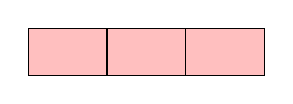
\begin{tikzpicture}[x=1mm,y=1mm,scale=.5]
\draw[fill=pink] (0,0) rectangle (60,12);
\foreach \x in {1,2} \draw (\x*60/3,0) -- (\x*60/3,12);
    \end{tikzpicture}        & \centering       3  & \parbox[t][1.3 
cm][c]{1cm}{$\frac{1}{3}$ } \\
    \hline
    \centering  \begin{tikzpicture}[x=1mm,y=1mm,scale=.5]
\draw[fill=special] (0,0) rectangle (60,12);
\foreach \x in {1,2,3} \draw (\x*60/4,0) -- (\x*60/4,12);
    \end{tikzpicture}        & \centering   4  &  \parbox[t][1.3 
cm][c]{1cm}{$\frac{1}{4}$}  \\
    \hline
 \centering  \begin{tikzpicture}[x=1mm,y=1mm,scale=.5]
\draw[fill=attention] (0,0) rectangle (60,12);
\foreach \x in {1,...,4} \draw (\x*60/5,0) -- (\x*60/5,12);
    \end{tikzpicture}        & \centering  5  & \parbox[t][1.3 
cm][c]{1cm}{$\frac{1}{5}$}  \\
    \hline
 \centering  \begin{tikzpicture}[x=1mm,y=1mm,scale=.5]
\draw[fill=common] (0,0) rectangle (60,12);
\foreach \x in {1,...,5} \draw (\x*60/6,0) -- (\x*60/6,12);
    \end{tikzpicture}        & \centering   6  & \parbox[t][1.3 
cm][c]{1cm}{$\frac{1}{6}$}  \\
    \hline
  \centering  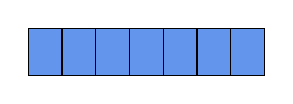
\begin{tikzpicture}[x=1mm,y=1mm,scale=.5]
\draw[fill=CornflowerBlue] (0,0) rectangle (60,12);
\foreach \x in {1,...,6} \draw (\x*60/7,0) -- (\x*60/7,12);
    \end{tikzpicture}        & \centering    7  & \parbox[t][1.3 
cm][c]{1cm}{$\frac{1}{7}$}  \\
    \hline
 \centering  \begin{tikzpicture}[x=1mm,y=1mm,scale=.5]
\draw[fill=dark] (0,0) rectangle (60,12);
\foreach \x in {1,...,7} \draw (\x*60/8,0) -- (\x*60/8,12);
    \end{tikzpicture}        & \centering  8  & \parbox[t][1.3 
cm][c]{1cm}{$\frac{1}{8}$}  \\
    \hline
 \centering  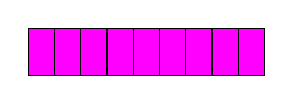
\begin{tikzpicture}[x=1mm,y=1mm,scale=.5]
\draw[fill=Fuchsia] (0,0) rectangle (60,12);
\foreach \x in {1,...,8} \draw (\x*60/9,0) -- (\x*60/9,12);
    \end{tikzpicture}        & \centering   9  & \parbox[t][1.3 
cm][c]{1cm}{$\frac{1}{9}$}  \\
    \hline
 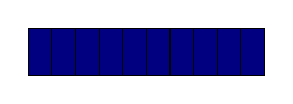
\begin{tikzpicture}   [x=1mm,y=1mm,scale=.5]
 \draw[fill=NavyBlue] (0,0) rectangle (60,12);
 \foreach \x in {1,...,9} \draw (\x*60/10,0) -- (\x*60/10,12);
     \end{tikzpicture}        & \centering     10  & \parbox[t][1.3 
cm][c]{1cm}{$\frac{1}{10}$}  \\
    \hline
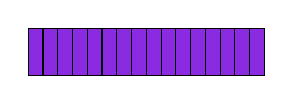
\begin{tikzpicture}   [x=1mm,y=1mm,scale=.5]
    \draw[fill=BlueViolet] (0,0) rectangle (60,12);
\foreach \x in {1,...,15} \draw (\x*60/16,0) -- (\x*60/16,12);
    \end{tikzpicture}        & \centering  16  & \parbox[t][1.3 
cm][c]{1cm}{$\frac{1}{16}$}  \\
    \hline 
 \end{tabular}
\end{center}  
  
  \pagebreak
  {\bf PARTE 2 }  
  
\noindent\begin{tabular}{|m{.15\textwidth}|m{.065\textwidth}|m{.07\textwidth}|m{
.075\textwidth}|}
 \hline
 \centering Tipo da peça &   Quantas cabem na região cinza? &   Juntas, são que 
fração do retângulo do encarte?  &  Fração do encarte não colorida de cinza? \\
    \hline    \hline
 \begin{tikzpicture}[x=1mm, y=1mm, scale=.5]
% Fita de largura 1/2
\draw[fill=light] (0,0) rectangle (100/2,10);
\end{tikzpicture} &  \parbox[t][1.3 cm][c]{1cm}{$1$} &  $\frac{1}{2}$ &  
$\frac{1}{2}$ \\
    \hline
\centering  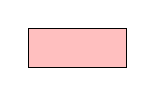
\begin{tikzpicture}[x=1mm, y=1mm, scale=.5]
% Fita rosa de largura 1/4
\draw[fill=pink] (0,0) rectangle (100/4,10);
\end{tikzpicture}
        &  \parbox[t][1.3 cm][c]{1cm}{ $2$ }  &  $\frac{2}{4}$ &  $\frac{2}{4}$ 
\\
    \hline
 \centering \begin{tikzpicture}[x=1mm, y=1mm, scale=.5]
% Fita rosa de largura 1/6
\draw[fill=special] (0,0) rectangle (100/6,10);
\end{tikzpicture}    &  \parbox[t][1.3 cm][c]{1cm}{ $3$ } &  $\frac{3}{6}$ &  
$\frac{3}{6}$ \\
    \hline
\centering \begin{tikzpicture}[x=1mm, y=1mm, scale=.5]
% Fita rosa de largura 1/8
\draw[fill=attention] (0,0) rectangle (100/8,10);
\end{tikzpicture}     &  \parbox[t][1.3 cm][c]{1cm}{   $4$} &  $\frac{4}{8}$ &  
$\frac{4}{8}$ \\
    \hline
\centering \begin{tikzpicture}[x=1mm, y=1mm, scale=.5]
% Fita rosa de largura 1/10
\draw[fill=common] (0,0) rectangle (100/10,10);
\end{tikzpicture}     &  \parbox[t][1.3 cm][c]{1cm}{ $5$ } &  $\frac{5}{10}$ &  
$\frac{5}{10}$ \\
    \hline
\centering 
\begin{tikzpicture}[x=1mm, y=1mm, scale=.5]
% Fita rosa de largura 1/16
\draw[fill=CornflowerBlue] (0,0) rectangle (100/16,10);
\end{tikzpicture}     &  \parbox[t][1.3 cm][c]{1cm}{ $8$ } &  $\frac{8}{16}$ &  
$\frac{8}{16}$ \\
    \hline
  \end{tabular}  
 
\end{resposta*}

\Bg

\subsection{Atividade 7}

 \noindent {\bf Objetivo específico: Levar o aluno a}  
\begin{itemize} %s
    \item       Reconhecer que, para cada       $0 \leq i \leq 3$, as frações    
   $\frac{i}{3}$,       $\frac{2 \times i}{2 \times 3 }$,       $\frac{3 \times 
i}{3 \times 3}$       e       $\frac{4 \times i}{4 \times 3}$       são iguais a 
partir da observação das representações destas frações na reta numérica.
\end{itemize} %s
  
  
  \noindent {\bf Recomendações e sugestões para o desenvolvimento da atividade:} 
 
\begin{itemize} %s
    \item       Recomenda-se que, nesta atividade, os alunos trabalhem 
individualmente ou em duplas. No entanto, é fundamental que os alunos sejam 
estimulados a explicar o raciocínio realizado.
    \item       Nas retas numéricas apresentadas, as origens estão alinhadas e 
as unidades correspondem a segmentos unitários congruentes, o que garante que 
uma fração associada a um determinado ponto em uma reta seja a mesma fração nos 
pontos correspondentes nas demais retas.
    \item       Caso seus alunos não percebam, aponte para o fato de que as 
segunda, terceira e quarta retas numéricas são obtidas por meio de subdivisões 
dos terços da primeira reta numérica em duas, três e quatro partes iguais, 
respectivamente. Para resolver o item c) desta atividade, se faz necessário 
dividir cada terço em cinco partes iguais.
    \item       É importante, ao final da atividade, observar para os alunos 
que, nesta atividade, cada ponto marcado na reta numérica está sendo descrito 
por frações com numeradores e denominadores diferentes (isto é, por frações 
equivalentes) mas que, não obstante, por corresponderem ao mesmo ponto da reta 
numérica, estas frações são iguais.
\end{itemize} %s
  
  
  Classificações:  
\begin{itemize} %s
    \item       Heid et al.: Conceito: identificar e descrever
    \item       Nicely, Jr.: Nível 1: reconhecer
    \item       UERJ: Observar: identificar e reconhecer
\end{itemize} %s
  
  
  Para o item c):  
\begin{itemize} %s
    \item       Heid et al.: Produto: gerar
    \item       Nicely, Jr.: Nível 3: comparar
    \item       UERJ: Interpretar: discriminar
\end{itemize} %s

\begin{resposta*}{Atividade 7}

\noindent a)

 \noindent \begin{tikzpicture}[x=45mm,y=45mm, scale=.53]
  \draw (0,0) -- (3,0);
  \foreach \x in {0,...,3}{ \draw (\x,-3pt) -- (\x, 3pt);  \node[above] at (\x,3pt) {\x}; }
  
  \foreach \x in {0,1,...,9}{
  \draw (\x/3,-2pt) -- (\x/3, 2pt);
  \node[below] at (\x/3,-2 pt) {$\frac{\x}{3}$};
  \draw[dotted] (\x/3,-35pt) -- (\x/3, -60pt);
  }
  
  \fill[common] (1+1/3,0) circle (2pt);
  
  \begin{scope}[shift={(0,-80pt)}]
  \draw (0,0) -- (3,0);
  \foreach \x in {0,...,3}{
  \draw (\x,-3pt) -- (\x, 3pt);
  \node[above] at (\x,3pt) {\x};
  }
  
  \foreach \x in {0,2,...,18}{ 
  \draw (\x/6,-2pt) -- (\x/6, 2pt);
  \node[below] at (\x/6,-2 pt) { $\frac{\x}{6}$ };
  \draw[dotted] (\x/6,-35pt) -- (\x/6, -60pt);
  }
  
  \foreach \x in {0,.333,...,6}{ 
  \draw (\x/2,-2pt) -- (\x/2, 2pt);}
  
  
  \fill[common] (1+1/3,0) circle (2pt);
   
  \end{scope}

  
  \begin{scope}[shift={(0,-160pt)}]
  \draw (0,0) -- (3,0);
  \foreach \x in {0,...,3}{ 
  \draw (\x,-3pt) -- (\x, 3pt);
  \node[above] at (\x,3pt) {\x};}
  
  \foreach \x in {0,3,...,27}{ 
  \draw (\x/9,-2pt) -- (\x/9, 2pt);
  \node[below] at (\x/9,-2 pt) {$\frac{\x}{9}$};
  \draw[dotted] (\x/9,-35pt) -- (\x/9, -60pt);
  }
  
  \foreach \x in {0,.333,...,9}{ 
  \draw (\x/3,-2pt) -- (\x/3, 2pt);}
  
  
  
  \fill[common] (1+1/3,0) circle (2pt);
   
  \end{scope}

  \begin{scope}[shift={(0,-240pt)}]
  \draw (0,0) -- (3,0);
  \foreach \x in {0,...,3}{ 
  \draw (\x,-3pt) -- (\x, 3pt);
  \node[above] at (\x,3pt) {\x};}
  
  \foreach \x in {0,4,...,36}{ 
  \draw (\x/12,-2pt) -- (\x/12, 2pt);
  \node[below] at (\x/12,-2 pt) {$\frac{\x}{12}$};
  %\draw[dotted] (\x,-30pt) -- (\x, -60pt);
  }
  
  \foreach \x in {0,.333,...,12}{ 
  \draw (\x/4,-2pt) -- (\x/4, 2pt);}
  
  \fill[common] (1+1/3,0) circle (2pt);
   
  \end{scope} 
 \end{tikzpicture}

\noindent b) $\frac{4}{3} = \frac{8}{6} = \frac{12}{9} = \frac{16}{12}$.

\noindent c) No item b) foi estabelecido que o ponto azul corresponde a fração       
$\frac{4}{3}$       pois, ao se justapor 4 segmentos que são       $\frac{1}{3}$ 
      do segmento unitário (que está, aqui, servindo como unidade) a partir da 
origem       $0$, este ponto é a outra extremidade desta justaposição. Agora, ao 
se subdividir estes 4 segmentos que são       $\frac{1}{3}$       do segmento 
unitário em 5 partes iguais, obtêm-se 20 segmentos justapostos que são       
$\frac{1}{15}$       do segmento unitário. Sendo o ponto azul extremo desta 
justaposição, segue-se que ele corresponde a fração       $\frac{20}{15}$.

  

\noindent \begin{tikzpicture}[x=45mm,y=45mm, scale=.53]
  \draw (0,0) -- (3,0);
  \foreach \x in {0,...,3}{ \draw (\x,-3pt) -- (\x, 3pt);  \node[above] at (\x,3pt) {\x}; }
  
  \foreach \x in {0,1,...,9}{
  \draw (\x/3,-2pt) -- (\x/3, 2pt);
  \node[below] at (\x/3,-2 pt) {$\frac{\x}{3}$};
  \draw[dotted] (\x/3,-35pt) -- (\x/3, -60pt);
  }
  
  \fill[common] (1+1/3,0) circle (2pt);
  
  \begin{scope}[shift={(0,-80pt)}]
  \draw (0,0) -- (3,0);
  \foreach \x in {0,...,3}{
  \draw (\x,-3pt) -- (\x, 3pt);
  \node[above] at (\x,3pt) {\x};
  }
  
  \foreach \x in {0,5,...,45}{ 
  \node[below] at (\x/15,-2 pt) { $\frac{\x}{15}$ };
  %\draw[dotted] (\x/15,-35pt) -- (\x/15, -60pt);
  }
  
  \foreach \x in {0,1,...,45}{ 
  \draw (\x/15,-2pt) -- (\x/15, 2pt);}
  
  
  \fill[common] (1+1/3,0) circle (2pt);
   
  \end{scope}
\end{tikzpicture}
  
\end{resposta*}

\Bg
\Bg
\Bg

\subsection{Atividade 8}

 \noindent {\bf Objetivo específico: Levar o aluno a}  
\begin{itemize} %s
    \item       Determinar uma fração igual a uma dada fração com denominador 
especificado a partir da observação das representações destas frações em 
diversos modelos de frações, incluindo a reta numérica.
\end{itemize} %s
  
  \noindent {\bf Recomendações e sugestões para o desenvolvimento da atividade:} 
 
\begin{itemize} %s
    \item       Recomenda-se que esta atividade seja desenvolvida em grupos de 3 
alunos (cada aluno do grupo poderá usar um modelo diferente para obter a fração 
solicitada).
    \item       É importante, ao final da atividade, observar para os alunos que 
uma mesma parte em cada modelo de área e um mesmo ponto na reta numérica estão 
sendo descritos por frações com numeradores e denominadores diferentes (isto é, 
por frações equivalentes) mas que, não obstante, estas frações são iguais por 
expressarem uma mesma quantidade ou por serem representadas por um mesmo ponto 
na reta numérica. 
\end{itemize} %s
  
  Classificações  
\begin{itemize} %s
    \item       Heid et al.: Produto: gerar
    \item       Nicely, Jr.: Nível 5: aplicar
    \item       UERJ: Interpretar: discriminar
\end{itemize} %s

\begin{resposta*}{Atividade 8}  
\begin{enumerate} [\quad a)] %s
    \item       Tomando um círculo como unidade, o dividimos em       $4$       
partes iguais e tomamos       $5$       cópias de uma parte para obter       
$\frac{5}{4}$       da unidade. Dividindo cada uma das       $5$       cópias em 
      $3$       partes iguais, obtemos então       $15$       cópias de       
$\frac{1}{12}$       da unidade. Portanto,       $\frac{5}{4} = \frac{15}{12}$.  
     
  

\noindent \begin{tikzpicture}[x=1mm,y=1mm, scale=1.45]
 \draw[fill=common, fill opacity=.3] (0,0) circle (5);
 \node at (0,7) {Unidade};
 

 \begin{scope}[xshift=45] 
 \draw[->] (-10,0) -- (-6,0);
 \node[text width=23 mm] at (-8,-10) {Divide-se a unidade em 4 partes iguais.}; 
 
 
 \draw[fill=common, fill opacity=.3] (0,0) circle (5);
 \draw (90:5) -- (-90:5);
 \draw (0:5) -- (180:5);
 
 \draw[->] (6,0) -- (10,0);
 \node[text width=20 mm] at (8,-12) {Uma parte corresponde a um quarto.}; 
 
 \draw[fill=common, fill opacity=.3, xshift=32, yshift=-5] (0:5) arc (0:90:5) -- (0,0)--cycle;
 
 \end{scope}
  
 \begin{scope}[ yshift=-23mm] 
 
 \node[text width=30 mm] at (3,-10) {Junta-se 5 cópias de uma parte para obter cinco quartos.};
 
 \draw[fill=common, fill opacity=.3] (0,0) circle (5);
 \draw (90:5) -- (-90:5);
 \draw (0:5) -- (180:5);
 
 \draw[fill=common, fill opacity=.3, xshift=6mm, yshift=-5] (0:5) arc (0:90:5) -- (0,0)--cycle;
 
 
 \begin{scope}[xshift=65] 
  \draw[->] (-10,0) -- (-6,0);
 \node[text width=33 mm] at (4,-12) {Divide-se cada cópia em 3 partes iguais obtendo 15 cópias de um doze avos.};
 
 \draw[fill=common, fill opacity=.3] (0,0) circle (5);
 \foreach \x in {0,30,...,150}{ \draw (\x:5) -- (\x:-5);}
  
 \draw[fill=common, fill opacity=.3, xshift=6mm, yshift=-5] (0:5) arc (0:90:5) -- (0,0)--cycle;
 \foreach \x in {30,60}{ \draw[xshift=6mm, yshift=-5] (\x:5) -- (0,0);}
 \end{scope}
 \end{scope}
 
 \end{tikzpicture}

    \item       Tomando um quadrado como unidade, o dividimos em       $4$       
partes iguais e tomamos       $5$       cópias de uma parte para obter       
$\frac{5}{4}$       da unidade. Dividindo cada uma das       $5$       cópias em 
      $3$       partes iguais, obtemos então       $15$       cópias de       
$\frac{1}{12}$       da unidade. Portanto,       $\frac{5}{4} = \frac{15}{12}$.  

\noindent \begin{tikzpicture}[x=1mm,y=1mm,scale=1.45]
           \draw[fill=common, fill opacity=.3] (0,0) rectangle (10,10);
	   \node at (5,12) {Unidade};
 
 
 \begin{scope}[xshift=45] 
 \draw[->] (-5,5) -- (-1,5);
 \node[text width=20 mm] at (-4,-6) {Divide-se a unidade em 4 partes iguais.}; 
 
 \draw[fill=common, fill opacity=.3] (0,0) rectangle (10,10);
 \draw (0,5) -- (10,5);
 \draw (5,0) -- (5,10);
 
 \draw[->] (11,5) -- (15,5);
 \node[text width=20 mm] at (12,-6) {Uma parte corresponde a um quarto.}; 
 
 \draw[fill=common, fill opacity=.3, xshift=16mm, yshift=2.5mm] (0,0) rectangle (5,5);
 
 \end{scope}
  
 \begin{scope}[ yshift=-23mm] 
 
 \node[text width=30 mm] at (10,-6) {Junta-se 5 cópias de uma parte para obter cinco quartos.};
 
 \draw[fill=common, fill opacity=.3] (0,0) rectangle (10,10);
 \draw (0,5) -- (10,5);
 \draw (5,0) -- (5,10);
 
 \draw[fill=common, fill opacity=.3, xshift=11mm, yshift=5mm] (0,0) rectangle (5,5);
 
 \draw[->] (17,5) -- (21,5);
 \begin{scope}[xshift=62] 

  \node[text width=30 mm] at (10,-9) {Divide-se cada cópia em 3 partes iguais obtendo 15 cópias de um doze avos.};
 
 \draw[fill=common, fill opacity=.3] (0,0) rectangle (10,10);
 \foreach \x in {10,20,...,50} \draw (\x/6,0) -- (\x/6,10);
 \draw (0,5) -- (10,5);
 
 \draw[fill=common, fill opacity=.3, xshift=11mm, yshift=5mm] (0,0) rectangle (5,5);
 \foreach \x in {10,20} \draw[xshift=11mm, yshift=5mm] (\x/6,0) -- (\x/6,5);
 \end{scope}
 \end{scope}
 
          \end{tikzpicture}


\end{enumerate} %s
\end{resposta*}          
          
\pagebreak
\end{multicols}
\begin{enumerate}[a)]

    \item[c)] Após marcar os números       $0$       e       $1$       na reta 
numérica, dividimos o segmento unitário (aquele de extremidades em       $0$     
  e       $1$) em       $4$       partes iguais. Cada parte é um segmento que 
corresponde a       $\frac{1}{4}$       da unidade. Ao se justapor       $5$     
  segmentos que são       $\frac{1}{4}$       da unidade a partir da origem 0, a 
fração       $\frac{5}{4}$       corresponde ao ponto que é a outra extremidade 
desta justaposição. Agora, ao se subdividir estes 5 segmentos que são       
$\frac{1}{4}$       da unidade em 5 partes iguais, obtêm-se       $15$       
segmentos justapostos que são       $\frac{1}{12}$       da unidade. O ponto que 
corresponde a       $\frac{5}{4}$       é ainda extremo desta justaposição e, 
portanto, que ele corresponde também a fração       $\frac{15}{12}$.      



\begin{center}
 
 \begin{tikzpicture}[x=21mm,y=21mm]
  \draw (0,0) -- (3,0);
  \foreach \x in {0,...,3}{ \draw (\x,-3pt) -- (\x, 3pt);  \node[above] at (\x,3pt) {\x}; }
  
  \foreach \x in {0,1,...,5}{
  \draw (\x/4,-2pt) -- (\x/4, 2pt);
  \node[below] at (\x/4,-2 pt) {$\frac{\x}{4}$};}
  \draw[dotted] (5/4,-.3) -- (5/4, -.6);
  
  
  \fill[common] (1+1/3,0) circle (2pt);
  
  \begin{scope}[shift={(0,-.7)}]
  \draw (0,0) -- (3,0);
  \foreach \x in {0,...,3}{
  \draw (\x,-3pt) -- (\x, 3pt);
  \node[above] at (\x,3pt) {\x};
  }
  
  \foreach \x in {0,3,...,15}{ 
  \node[below] at (\x/12,-2 pt) { $\frac{\x}{12}$ };
  %\draw[dotted] (\x/15,-35pt) -- (\x/15, -60pt);
  }
  
  \foreach \x in {0,1,...,15}{ 
  \draw (\x/12,-2pt) -- (\x/12, 2pt);}
  
  
  \fill[common] (1+1/4,0) circle (2pt);
   
  \end{scope}
\end{tikzpicture}

\end{center}
\end{enumerate}
\pagebreak

\begin{multicols}{2}
\subsection{Atividade 9}

 \noindent {\bf Objetivo específico: Levar o aluno a}  
\begin{itemize} %s
    \item       Determinar uma fração igual a uma dada fração irredutível com 
denominador especificado.
\end{itemize} %s
  
  
  \noindent {\bf Recomendações e sugestões para o desenvolvimento da atividade:} 
 
  
\begin{itemize} %s
    \item       Recomenda-se que, nesta atividade, os alunos trabalhem 
individualmente ou em duplas. No entanto, é fundamental que os alunos sejam 
estimulados a explicar o raciocínio realizado.
    \item       Espera-se, principalmente nos Itens c e d, que os alunos 
consigam obter a fração solicitada usando a propriedade que       $\frac{m 
\times a}{m \times b}$       é equivalente a       $\frac{a}{b}$       e sem 
recorrer a desenhos de modelos de área de frações.
\end{itemize} %s
  
  
  Classificações  
\begin{itemize} %s
    \item       Heid et al.: Produto: gerar
    \item       Nicely, Jr.: Nível 3: comparar
    \item       UERJ: Interpretar: discriminar
\end{itemize} %s


\begin{resposta*}{Atividade 9}
\begin{enumerate} [\quad a)] %s
    \item       Como       $6 = 2 \times 3$, segue-se que       $\frac{7}{3} = 
\frac{2 \times 7}{2 \times 3} = \frac{14}{6}$.
    \item       Como       $21 = 7 \times 3$, segue-se que       $\frac{7}{3} = 
\frac{7 \times 7}{7 \times 3} = \frac{49}{21}$.
    \item       Como       $123 = 41 \times 3$, segue-se que       $\frac{7}{3} 
= \frac{41 \times 7}{41 \times 3} = \frac{287}{123}$.
    \item       Como       $210 = 70 \times 3$, segue-se que       $\frac{7}{3} 
= \frac{70 \times 7}{70 \times 3} = \frac{490}{210}$.
\end{enumerate} %s
\end{resposta*}

\subsection{Atividade 10}

 \noindent {\bf Objetivo específico: Levar o aluno a}  
\begin{itemize} %s
    \item       Determinar uma fração igual a uma dada fração com numerador ou 
denominador especificados.
\end{itemize} %s
  
\noindent {\bf Recomendações e sugestões para o desenvolvimento da atividade:}  
\begin{itemize} %s
    \item       Recomenda-se que, nesta atividade, os alunos trabalhem 
individualmente. No entanto, é fundamental que os alunos sejam estimulados a 
explicar o raciocínio realizado.
    \item       Espera-se que, neste estágio, os alunos consigam obter as 
respostas usando a propriedade que       $\frac{m \times a}{m \times b}$       é 
equivalente a       $\frac{a}{b}$       e sem recorrer a desenhos de modelos de 
área de frações.
    \item       Observe que, no item (e), não existe um número natural       $n$ 
      tal que       $6 \times n = 9$. Para resolver o item, o aluno pode usar o 
resultado do item (d) e substituir       $\frac{9}{12}$       por       
$\frac{3}{4}$       e proceder com o exercício. A mesma observação aplica-se ao 
item (f).
    \item       Observe para seus alunos que os Itens (e) e (f) são exemplos de 
frações iguais para os quais não é possível obter uma fração multiplicando-se o 
numerador e o denominador da outra por um mesmo número natural.
\end{itemize} %s
  
  
  Classificações  
\begin{itemize} %s
    \item       Heid et al.: Produto: gerar
    \item       Nicely, Jr.: Nível 3: comparar
    \item       UERJ: Interpretar: discriminar
\end{itemize} %s
  

\begin{resposta*}{Atividade 10} 
\begin{enumerate} [\quad a)] %s
    \item       Uma vez que       $6 = 2 \times 3$, então       $\frac{5}{3} = 
\frac{2 \times 5}{2 \times 3} = \frac{10}{6}$. Logo,       $\square$       deve 
ser preenchido com       $10$.
    \item       Uma vez que       $6 = 3 \times 2$, então       $\frac{2}{3} = 
\frac{3 \times 2}{3 \times 3} = \frac{6}{9}$. Logo,       $\square$       deve 
ser preenchido com       $9$.
    \item       Uma vez que       $12 = 4 \times 3$       e       $8 = 4 \times 
2$, então       $\frac{8}{12} = \frac{4 \times 2}{4 \times 3} = \frac{2}{3}$. 
Logo,       $\square$       deve ser preenchido com       $2$.
    \item       Uma vez que       $9 = 3 \times 3$       e       $12 = 3 \times 
4$, então       $\frac{9}{12} = \frac{3 \times 3}{3 \times 4} = \frac{3}{4}$. 
Logo,       $\square$       deve ser preenchido com       $4$.
    \item       Pelo item d,       $\frac{9}{12} = \frac{3}{4}$. Uma vez que     
  $6 = 2 \times 3$, então       $\frac{3}{4} = \frac{2 \times 3}{2 \times 4} = 
\frac{6}{8}$. Logo,       $\square$       deve ser preenchido com       $8$.
    \item       Pela solução do item e,       $\square$       deve ser 
preenchido com       $9$.
\end{enumerate} %s
  
\end{resposta*}



\subsection{Atividade 11}

 \noindent {\bf Objetivo específico: Levar o aluno a}  
\begin{itemize} %s
    \item       Usar igualdade de frações para calcular o numerador de uma das 
frações em uma situação contextualizada.
\end{itemize} %s
  
  \noindent {\bf Recomendações e sugestões para o desenvolvimento da atividade:} 
 
\begin{itemize} %s
    \item       Recomenda-se que, nesta atividade, os alunos trabalhem 
individualmente ou em duplas. No entanto, é fundamental que os alunos sejam 
estimulados a explicar o raciocínio realizado.
\end{itemize} %s

Classificações
\begin{itemize} %s
  \item     Heid et al.: Produto: prever
  \item     Nicely, Jr.: Nível 6: analisar
  \item     UERJ: Interpretar: explicar
\end{itemize} %s

\begin{resposta*}{Atividade 11}  
  As 17 marcações no copo do seu colega divide a capacidade do copo em 16 partes 
iguais. Quantas destas partes correspondem a   $\frac{3}{4}$   da capacidade do 
copo (que é fração da capacidade do copo que está preenchida com suco)? Para 
responder a esta pergunta, devemos calcular o numerador de uma fração de 
denominador 16 que seja igual a   $\frac{3}{4}$  , isto é, devemos preencher   
$\square$   com um número tal que  
  
  $\frac{3}{4} = \frac{\square}{16}$.  
  
  Como   $16 = 4 \times 4$  , segue-se que  
  
  $\frac{3}{4} = \frac{4 \times 3}{4 \times 4} = \frac{12}{16}$.   
  
  Assim, não necessárias   $12$   partes de   $\frac{1}{16}$   da capacidade do 
copo. Consequentemente,  
  13 níveis do copo do seu colega devem ser preenchidos com suco de laranja para 
que ele fique com a mesma quantidade suco de laranja que você.  
  

\begin{center}
 \begin{tikzpicture}[scale=0.5, x=1cm,y=1cm]
 
% Definição do eixo vertical das elipses
\def\EixoM{0.3}

% colorindo o primeiro cilindro
\fill[light, opacity=1] (2,0) ellipse (2 and \EixoM);
\fill[light,fill opacity=.8] (0,0) rectangle (4,3);
\fill[fill=light,fill opacity=1] (2,3) ellipse (2 and \EixoM);


\pgfpathmoveto{\pgfpoint{0 cm}{0 cm}}
\pgfpatharc{-180}{0}{2cm and \EixoM cm}
\pgfusepath{draw}

\draw (2,4) ellipse (2 and \EixoM);
\draw (0,0) -- (0,4);
\draw (4,0) -- (4,4);

% shift vertical nos arcos de elipse definido por \y
\foreach \y in {0,.25,...,4}{
\pgfpathmoveto{\pgfpoint{0 cm}{\y cm}}
\pgfpatharc{-180}{-130}{2cm and \EixoM cm}
\color{Green}
\pgfusepath{draw}}
\end{tikzpicture}
\end{center}

 \end{resposta*}




\subsection{Atividade 12}

 \noindent {\bf Objetivo específico: Levar o aluno a}  
\begin{itemize} %s
    \item       Reconhecer que, dada uma fração       $p = \frac{n}{d}$, existe 
um quantidade finita de frações da forma       $\frac{k}{d}$       que são 
menores do que       $p$       e uma quantidade infinita de frações da forma     
  $\frac{k}{d}$       que são maiores do que       $p$.
\end{itemize} %s
  
  
  \noindent {\bf Recomendações e sugestões para o desenvolvimento da atividade:} 
 
\begin{itemize} %s
    \item       Recomenda-se que, nesta atividade, os alunos trabalhem 
individualmente ou em duplas. No entanto, é fundamental que os alunos sejam 
estimulados a explicar o raciocínio realizado.
    \item       Alguns alunos podem ainda necessitar de apoio de material 
concreto para responder à questão.
    \item       Recomenda-se que, na discussão da atividade, uma reta numérica 
com quintos marcados seja usada como uma contrapartida visual para as respostas 
das perguntas.
\end{itemize} %s
  

\noindent \begin{tikzpicture}[x=23mm,y=23mm]
  \draw[->] (-0.1,0) -- (3.1,0);
  \foreach \x in {0,...,3}{ \draw (\x,-3pt) -- (\x, 3pt);  \node[above] at (\x,3pt) {\x}; }
  
  \foreach \x in {0,1,...,15}{
  \draw (\x/5,-2pt) -- (\x/5, 2pt);
  \node[below] at (\x/5,-2 pt) {$\frac{\x}{5}$};}
    
  \fill[common] (3/5,0) circle (2pt);
  \end{tikzpicture}
  
  
Classificações  
\begin{itemize} %s
    \item       Heid et al.: Conceito: elaborar
    \item       Nicely, Jr.: Nível 4: categorizar
    \item       UERJ: Interpretar: classificar
\end{itemize} %s
  

\begin{resposta*}{Atividade 12}  
\begin{enumerate} [\quad a)] %d
    \item       Três frações:       $\frac{0}{5}$,       $\frac{1}{5}$       e   
    $\frac{2}{5}$. Justificativa:       $\frac{3}{5}$       são três       
``cópias''       de       $\frac{1}{5}$. Qualquer outra fração de denominador    
   $5$       também é composta por uma quantidade inteira de       ``cópias''    
   de       $\frac{1}{5}$, quantidade esta determinada pelo numerador de fração. 
Para se ter então uma fração de denominador       $5$       menor do que       
$\frac{3}{5}$, devemos ter menos do que       $3$             ``cópias''       
de       $\frac{1}{5}$      :       $2$             ``cópias''      ,       $1$  
           ``cópia''       ou       $0$             ``cópia''      . Assim, as 
frações de denominador       $5$       menor do que       $\frac{3}{5}$       
são       $\frac{0}{5}$,       $\frac{1}{5}$       e       $\frac{2}{5}$. 
    \item       Infinitas frações       $\frac{4}{5}$,       $\frac{5}{5}$,      
 $\frac{6}{5}$,       $\frac{7}{5}$, etc. Justificativa:       $\frac{3}{5}$     
  são três       ``cópias''       de       $\frac{1}{5}$. Qualquer outra fração 
de denominador       $5$       também é composta por uma quantidade inteira de   
    ``cópias''       de       $\frac{1}{5}$, quantidade esta determinada pelo 
numerador de fração. Para se ter então uma fração de denominador       $5$       
maior do que       $\frac{3}{5}$, devemos ter mais do que       $3$             
``cópias''       de       $\frac{1}{5}$      :       $4$             ``cópias''  
    ,       $5$             ``cópias''      ,       $6$             ``cópias''   
   ,       $7$             ``cópias''      , etc. Assim, as frações de 
denominador       $5$       maiores do que       $\frac{3}{5}$       são       
$\frac{4}{5}$,       $\frac{5}{5}$,       $\frac{6}{5}$,       $\frac{7}{5}$, 
etc.
\end{enumerate} %d
  
\end{resposta*}



\subsection{Atividade 13}

 \noindent {\bf Objetivo específico: Levar o aluno a}  
\begin{itemize} %s
    \item       Comparar frações por meio de igualdade de frações.
\end{itemize} %s
  
  
  \noindent {\bf Recomendações e sugestões para o desenvolvimento da atividade:} 
 
\begin{itemize} %s
    \item       Esta é uma atividade que pode ser desenvolvida individualmente. 
Contudo, é fundamental que os alunos sejam estimulados a explicar o raciocínio 
realizado.
    \item       A discussão da atividade pode incluir o uso de outras 
estratégias, que não a igualdade de frações, para se estabelecer a comparação 
das frações apresentadas. 
\end{itemize} %s
  
  
  Classificações  
\begin{itemize} %s
    \item       Heid et al.: Conceito: elaborar
    \item       Nicely, Jr.: Nível 3: comparar
    \item       UERJ: Interpretar: comparar
\end{itemize} %s

\begin{resposta*}{Atividade 13}
  
\noindent
    \begin{tabular}{lrcl}
      
       item &  Fração &  ``$>$'', ``$<$'' ou ``$=$'' &  Fração \\
      \hline 
       a) &  $\frac{5}{6} = \frac{25}{30}$ &   $>$  &  $\frac{24}{30} = 
\frac{4}{5}$ \\
     
       b) &  $\frac{3}{4} = \frac{9}{12}$ &   $>$  &  $\frac{8}{12} = 
\frac{2}{3}$ \\
     
       c) &  $\frac{2}{10} = \frac{1}{5}$ &   $=$  &  $\frac{1}{5} = 
\frac{3}{15}$ \\
     
       d) &  $\frac{6}{25} = \frac{24}{100}$ &   $<$  &  $\frac{25}{100} = 
\frac{1}{4}$ \\
     
       e) &  $\frac{22}{7} = \frac{220}{70}$ &   $>$  &  $\frac{217}{70} = 
\frac{31}{10}$ \\
     
       f) &  $\frac{22}{33} = \frac{2}{3}$ &   $=$  &  $\frac{2}{3} = 
\frac{24}{36}$ \\
     
       g) &  $\frac{5}{10} = \frac{50}{100}$ &   $=$  &  $\frac{50}{100} = 
\frac{50}{100}$ \\
     
       h) &  $\frac{7}{5} = \frac{84}{60}$ &   $<$  &  $\frac{85}{60} = 
\frac{17}{12}$ \\
     
       i) &  $\frac{12}{6} = \frac{2}{1}$ &   $<$  &  $\frac{3}{1} = 
\frac{9}{3}$ \\
      
    \end{tabular}
\end{resposta*}

\clearpage

\subsection{Atividade 14}

 \noindent {\bf Objetivo específico: Levar o aluno a}  
\begin{itemize} %s
    \item       Comparar frações.
\end{itemize} %s
  
  
  \noindent {\bf Recomendações e sugestões para o desenvolvimento da atividade:} 
 
\begin{itemize} %s
    \item       Recomenda-se que, nesta atividade, os alunos trabalhem 
individualmente ou em duplas. No entanto, é fundamental que os alunos sejam 
estimulados a explicar o raciocínio realizado.
    \item       Existem outros tipos de ferramentas cujas peças componentes 
também são identificadas por frações: brocas de furadeiras, chaves de boca e 
aperto, chaves biela,       $\ldots$
    \item       Recomenda-se que, caso seja viável, algumas destas ferramentas 
sejam levadas para sala de aula para conhecimento dos alunos.
\end{itemize} %s
  
  
  Classificações  
\begin{itemize} %s
    \item       Heid et al.: Conceito: elaborar
    \item       Nicely, Jr.: Nível 3: comparar
    \item       UERJ: Interpretar: comparar
\end{itemize} %s

\begin{resposta*}{Atividade 14}
  Uma vez que   $\frac{1}{2} = \frac{8}{16}$  ,   $\frac{3}{4} = \frac{12}{16}$  
,   $\frac{3}{8} = \frac{6}{16}$  ,   $\frac{5}{8} = \frac{10}{16}$   e   
$\frac{7}{8} = \frac{14}{16}$  , os tamanhos dos soquetes são os seguintes:  
  
  (A):   $\frac{7}{8}$  ,  
  (B):   $\frac{13}{16}$  ,  
  (C):   $\frac{3}{4}$  ,   
  (D):   $\frac{11}{16}$  ,  
  (E):   $\frac{5}{8}$  ,  
  (F):   $\frac{9}{16}$  ,  
  (G):   $\frac{1}{2}$  ,  
  (H):   $\frac{7}{16}$  ,  
  (I):   $\frac{3}{8}$.  
\end{resposta*}



\subsection{Atividade 15}

 \noindent {\bf Objetivo específico: Levar o aluno a}  
\begin{itemize} %s
    \item       Comparar uma fração com uma outra fração determinada a partir da 
alteração dos termos (numerador ou denominador) da primeira fração a partir de 
somas e multiplicações por números naturais.
\end{itemize} %s
  
  
  \noindent {\bf Recomendações e sugestões para o desenvolvimento da atividade:} 
 
\begin{itemize} %s
    \item       Recomenda-se que, nesta atividade, os alunos trabalhem 
individualmente ou em duplas. No entanto, é fundamental que os alunos sejam 
estimulados a explicar o raciocínio realizado.
    \item       Enquanto que esta atividade usa a fração       $\frac{4}{7}$     
  como referência, a discussão da atividade com os alunos pode incluir a questão 
se as conclusões obtidas para       $\frac{4}{7}$       mudam se a fração de 
referência mudar. Neste contexto, o item (D) é especialmente interessante pois, 
neste caso, a conclusão (se a fração ficará menor, maior ou igual a fração 
original) de fato dependerá se a fração original é maior, menor ou igual a       
$1$.
\end{itemize} %s
  
  
  Classificações  
\begin{itemize} %s
    \item       Heid et al.: Produto: prever
    \item       Nicely, Jr.: Nível 6: analisar
    \item       UERJ: Analisar: levantar hipóteses
\end{itemize} %s

\begin{resposta*}{Atividade 15}
\begin{enumerate} [\quad a)] %s
    \item       A fração determinada pela adição de 1 ao numerador da fração     
  $\frac{4}{7}$       é a fração       $\frac{5}{7}$       que é maior do que    
   $\frac{4}{7}$, pois em cinco sétimos temos um sétimo a mais do que em quatro 
sétimos.
    \item       A fração determinada pela adição de 1 ao denominador da fração   
    $\frac{4}{7}$       é a fração       $\frac{4}{8}$       que é menor do que  
     $\frac{4}{7}$, pois como um oitavo é menor do um sétimo, quatro oitavos 
também será menor do que quatro sétimos.
    \item       A fração determinada pela subtração de 1 ao denominador da 
fração       $\frac{4}{7}$       é a fração       $\frac{3}{7}$       que é 
menor do que       $\frac{4}{7}$, pois em três sétimos temos um sétimo a menos 
do que em quatro sétimos.
    \item       A fração determinada pela adição de 2 ao numerador e ao 
denominador da fração       $\frac{4}{7}$       é a fração       $\frac{6}{9}$   
    que é maior do que       $\frac{4}{7}$, pois       $\frac{6}{9} = 
\frac{2}{3} = \frac{7 \times 2}{7 \times 3} = \frac{14}{21}$,       $\frac{4}{7} 
= \frac{3 \times 4}{3 \times 7} = \frac{12}{21}$       e       $14 > 12$.
    \item       A fração determinada pela multiplicação por 2 do numerador e do 
denominador da fração       $\frac{4}{7}$       é a fração       $\frac{8}{14}$  
     que é igual a       $\frac{4}{7}$.
    \item       A fração determinada pela adição de 1 ao numerador e subtração 
de 1 ao denominador da fração       $\frac{4}{7}$       é a fração       
$\frac{5}{6}$       que é maior do que       $\frac{4}{7}$, pois       
$\frac{5}{6} > \frac{4}{6} > \frac{4}{7}$.
\end{enumerate} %s
  
  
\end{resposta*}



\subsection{Atividade 16}
  
 \noindent {\bf Objetivo específico: Levar o aluno a}  
\begin{itemize} %s
    \item       Obter uma fração irredutível equivalente a uma fração dada e 
relacionar esta equivalência no contexto de minimização de cortes em uma 
equipartição.
\end{itemize} %s
  
  \noindent {\bf Recomendações e sugestões para o desenvolvimento da atividade:} 
 
\begin{itemize} %s
    \item       Recomenda-se que, nesta atividade, os alunos trabalhem 
individualmente ou em duplas. No entanto, é fundamental que os alunos sejam 
estimulados a explicar o raciocínio realizado.
    \item       A discussão da atividade, além da equipartição dada e aquela 
associada ao número mínimo de cortes, pode incluir as equipartições associadas a 
outras frações equivalentes a       $\frac{8}{24}$      :       $\frac{4}{12}$   
    (divisão de cada panqueca em 12 partes iguais) e       $\frac{2}{6}$       
(divisão da panqueca em 6 partes iguais).
\end{itemize} %s
  
  
  Classificações  
\begin{itemize} %s
    \item       Heid et al.: Produto: prever
    \item       Nicely, Jr.: Nível 6: analisar
    \item       UERJ: Analisar: levantar hipóteses
\end{itemize} %s
  

\begin{resposta*}{Atividade 16}
\begin{enumerate} [\quad a)] %s
    \item       Cada amigo vai receber       $\frac{8}{24}$       de panqueca.
    \item             $8 \times 24 = 192$       cortes.
    \item       Sim! Por exemplo, como       $\frac{8}{24} = \frac{8 \times 1}{8 
\times 3} = \frac{1}{3}$, basta dividir cada panqueca       $3$       partes 
iguais e dar uma parte (      $\frac{1}{3}$       de panqueca para cada amigo. 
Para esta equipartição, são necessários       $8 \times 3 = 24$       cortes 
apenas.
\end{enumerate} %s
  
\end{resposta*}



\subsection{Atividade 17}

 \noindent {\bf Objetivo específico: Levar o aluno a}  
\begin{itemize} %s
    \item       Simplificar frações de modo a obter uma fração igual 
irredutível.
\end{itemize} %s
  
  \noindent {\bf Recomendações e sugestões para o desenvolvimento da atividade:} 
 
\begin{itemize} %s
    \item       Recomenda-se que, nesta atividade, os alunos trabalhem 
individualmente ou em duplas. No entanto, é fundamental que os alunos sejam 
estimulados a explicar o raciocínio realizado.
    \item       Um pré-requisito desta atividade é o conceito de máximo divisor 
comum. Assim, avalie a necessidade de uma revisão deste conceito com seus 
alunos. Os alunos devem perceber que se dois números são divididos pelo maior 
divior comum entre eles, os dois novos números obtidos são agora primos entre 
si, isto é, o máximo divisor comum entre eles é 1. Este fato vai apoiar o       
``assim''       das respostas. 
    \item       A discussão desta atividade pode incluir o uso de materiais 
concretos na linha da proposta da \emph{Atividade 16}      , isto é, relacionar  
frações equivalentes com a minimização de cortes em uma equipartição.
\end{itemize} %s
  
  Classificações  
\begin{itemize} %s
    \item       Heid et al.: Produto: gerar
    \item       Nicely, Jr.: Nível 3: comparar
    \item       UERJ: Interpretar: discriminar
\end{itemize} %s

\begin{resposta*}{Atividade 17}
\begin{enumerate}
 \item Note que o máximo divisor comum de   $2$   e   $4$   é 2. Assim,   
$\frac{2}{4} = \frac{2 \times 1}{2 \times 2} = \frac{1}{2}$. Resposta:   
$\frac{1}{2}$.  
 \item Note que o máximo divisor comum de   $6$   e   $3$   é 3. Assim,   
$\frac{6}{9} = \frac{3 \times 2}{3 \times 3} = \frac{2}{3}$. Resposta:   
$\frac{2}{3}$.  
 \item Note que o máximo divisor comum de   $2$   e   $4$   é 2. Assim,   
$\frac{4}{2} = \frac{2 \times 2}{2 \times 1} = \frac{2}{1}$. Resposta:   
$\frac{2}{1}$.  
 \item Note que o máximo divisor comum de   $5$   e   $35$   é 5. Assim,   
$\frac{5}{35} = \frac{5 \times 1}{5 \times 7} = \frac{1}{7}$. Resposta:   
$\frac{1}{7}$.  
 \item Note que o máximo divisor comum de   $50$   e   $100$   é 50. Assim,   
$\frac{50}{100} = \frac{50 \times 1}{50 \times 2} = \frac{1}{2}$. Resposta:   
$\frac{1}{2}$.  
\end{enumerate}

\end{resposta*}



\subsection{Atividade 18}
  
 \noindent {\bf Objetivo específico: Levar o aluno a}  
\begin{itemize} %s
    \item       Comparar mais do que duas frações (no caso, três) usando frações 
equivalentes.
\end{itemize} %s
  
  
  \noindent {\bf Recomendações e sugestões para o desenvolvimento da atividade:} 
 
\begin{itemize} %s
    \item       Esta é uma atividade que pode ser desenvolvida individualmente. 
Contudo, é fundamental que os alunos sejam estimulados a explicar o raciocínio 
realizado.
    \item       Sugere-se que seja observado para os alunos que o procedimento 
descrito nesta atividade para ordenar três frações pode ser aplicado para um 
número arbitrário de frações.
    \item       Esta atividade foi concebida para ser resolvida usando a notação 
de fração, sem o uso do recurso de modelos de frações uma vez que, neste 
estágio, espera-se que o aluno já tenha o domínio desta técnica de manipulação 
aritmética.
    \item       Observe que a ordenação poderia ser feita comparando-se duas 
frações por vez. A solução indicada reduz a ordenação à ordenação de números 
naturais (os numeradores das frações iguais às frações dadas e todas de mesmo 
denominador).
\end{itemize} %s
  
  
  Classificações  
\begin{itemize} %s
    \item       Heid et al.: Produto: gerar
    \item       Nicely, Jr.: Nível 3: comparar
    \item       UERJ: Interpretar: ordenar
\end{itemize} %s
  
\begin{resposta*}{Atividade 18}
\begin{enumerate} [\quad a)] %s
    \item             $60$       é um múltiplo comum de       $6$,       $20$    
   e       $15$      :       $60 = 10 \times 6$,       $60 = 4 \times 15$       
e       $60 = 3 \times 20$. Portanto,       $$\frac{11}{6} = \frac{10 \times 
11}{10 \times 6} = \frac{110}{60},$$             $$\frac{28}{15} = \frac{4 
\times 28}{4 \times 15} = \frac{112}{60} \quad {\rm  e}$$             
$$\frac{37}{20} = \frac{3 \times 37}{3 \times 20} = \frac{111}{60}.$$      
\mbox{} \newline 
    \item       Tem-se que       $\frac{110}{60} < \frac{111}{60} < 
\frac{112}{60}$. Logo,
\end{enumerate} %s
  
  $$\frac{11}{6} < \frac{37}{20} < \frac{28}{15}.$$  
\end{resposta*}

\subsection{Atividade 19}

 \noindent {\bf Objetivo específico: Levar o aluno a}  
\begin{itemize} %s
    \item       Verificar que se       $a \cdot d = b \cdot c$, com       $b 
\not = 0$       e       $d \not = 0$, então as frações       $\frac{a}{b}$       
e       $\frac{c}{d}$       são iguais (equivalentes).
\end{itemize} %s
  
  
  \noindent {\bf Recomendações e sugestões para o desenvolvimento da atividade:} 
 
\begin{itemize} %s
    \item       Esta é uma atividade que pode ser desenvolvida individualmente. 
Contudo, é fundamental que os alunos sejam estimulados a explicar o raciocínio 
realizado.
    \item       Note que para as frações usadas no exemplo e no item a), os 
numeradores e denominadores de uma fração não são múltiplos inteiros dos 
numeradores e denominadores da outra fração.
\end{itemize} %s
  
  
  Classificações  
\begin{itemize} %s
    \item       Heid et al.: Produto: descrever procedimento
    \item       Nicely, Jr.: Nível 5: aplicar
    \item       UERJ: Interpretar: compor e decompor
\end{itemize} %s

\begin{resposta*}{Atividade 19}  
\begin{enumerate} [\quad a)] %s
    \item       Para as frações       $\frac{2}{8}$       e       
$\frac{5}{20}$, tem-se que        $2 \times 20 = 40 = 8 \times 5$. Agora,       
$$\frac{2}{8} = \frac{20 \times 2}{20 \times 8} = \frac{2 \times 20}{20 \times 
8} = \frac{8 \times 5}{20 \times 8} = \frac{8 \times 5}{8 \times 20} = 
\frac{5}{20}.$$
    \item       A afirmação é verdadeira. 
  
  Ao se multiplicar o numerador e o denominador da primeira fração pelo 
denominador da segunda fração obtém-se uma fração de igual valor cujo numerador 
é o produto do numerador da primeira fração pelo denominador da segunda fração e 
cujo denominador é o produto do numerador da primeira fração pelo denominador da 
segunda fração.   
  
  Do mesmo modo, ao se multiplicar o numerador e o denominador da segunda fração 
pelo denominador da primeira fração obtém-se uma fração de igual valor cujo 
numerador é igual ao denominador da primeira fração multiplicado pelo numerador 
da segunda fração e cujo denominador é o produto do denominadora da primeira 
fração pelo denominador da segunda fração.   
  
  Como as frações iniciais são iguais, estas novas frações também são iguais e 
têm o mesmo denominador. Portanto, seus numeradores devem ser iguais, isto é, o 
produto do numerador da primeira fração pelo denominador da segunda fração é 
igual ao produto do denominador da primeira fração pelo numerador da segunda 
fração.  
\end{enumerate} %s

  \end{resposta*}


\subsection{Atividade 20}

 \noindent {\bf Objetivo específico: Levar o aluno a}  
\begin{itemize} %s
    \item       Reconhecer frações iguais por meio de um jogo de trilha.
\end{itemize} %s
  
  
  Esta atividade possui     folhas para reprodução disponíveis no final do 
livro.
  
  Classificações  
\begin{itemize} %s
    \item       Heid et al.: Produto: gerar; prever
    \item       Nicely, Jr.: Nível 5: relacionar
    \item       UERJ: Interpretar: ordenar
\end{itemize} %s
  
  \pagebreak
  
\subsection{Atividade 21}

 \noindent {\bf Objetivo específico: Levar o aluno a}  
\begin{itemize} %s
    \item       Perceber que mesmo se       $n < p$       e       $m < q$, pode 
ocorrer que       $\frac{n}{m} \geq \frac{p}{q}$.
\end{itemize} %s
  
  
  \noindent {\bf Recomendações e sugestões para o desenvolvimento da atividade:} 
  
\begin{itemize} %s
    \item       Esta é uma atividade que pode ser desenvolvida individualmente. 
Contudo, é fundamental que os alunos sejam estimulados a explicar o raciocínio 
realizado.
    \item       O tipo de situação descrita na atividade é um equívoco comum 
entre os alunos, isto é, eles equivocamente acham que se       $n < p$       e   
    $m < q$, então necessariamente       $\frac{n}{m} < \frac{p}{q}$.
\end{itemize} %s
  
  
  Classificações  
\begin{itemize} %s
    \item       Heid et al.: Raciocínio: corroborar
    \item       Nicely, Jr.: Nível 6: justificar
    \item       UERJ: Avaliar: julgar
\end{itemize} %s

\begin{resposta*}{Atividade 21}
  Tem-se que   $\frac{2}{3} = \frac{10 \times 2}{10 \times 3} = \frac{20}{30}$   
e  
  $\frac{6}{10} = \frac{3 \times 6}{3 \times 10} = \frac{18}{30}$.  
  Como   $\frac{20}{30} > \frac{18}{30}$  , segue-se que   $\frac{2}{3} > 
\frac{6}{10}$.  
\end{resposta*}

\subsection{Atividade 22}

 \noindent {\bf Objetivo específico: Levar o aluno a}  
\begin{itemize} %s
    \item       Analisar quando uma fração é igual a uma fração unitária.
\end{itemize} %s
  
  
  \noindent {\bf Recomendações e sugestões para o desenvolvimento da atividade:} 
 
\begin{itemize} %s
    \item       Esta é uma atividade que pode ser desenvolvida individualmente. 
Contudo, é fundamental que os alunos sejam estimulados a explicar o raciocínio 
realizado.
    \item       O item c) relaciona-se com a Atividade 1: como não é possível, 
em uma equipartição de uma região retangular, escolher uma quantidade de partes 
que corresponda à metade desta região se a quantidade total de partes for um 
número ímpar, não existe uma fração de denominador ímpar que seja igual à fração 
      $\frac{1}{2}$.
    \item       Observe para seus alunos que as frações estudadas na Lição 1 são 
justamente as frações unitárias e que, pela Lição 2, toda fração é a 
justaposição de frações unitárias. Em outras palavras, as frações unitárias 
constituem a estrutura básica a partir da qual as demais frações são obtidas.
\end{itemize} %s
  
  
  Classificações  
\begin{itemize} %s
    \item       Heid et al.: Raciocínio: corroborar
    \item       Nicely, Jr.: Nível 6: justificar
    \item       UERJ: Avaliar: julgar
\end{itemize} %s
  
\begin{resposta*}{Atividade 22}
\begin{enumerate} [\quad a)] %s
    \item       Pelo item b) da \emph{Atividade 19}      , se uma dada fração é 
igual a alguma fração unitária, então o produto do numerador da fração dada pelo 
denominador da fração unitária tem que ser igual ao denominador da fração dada, 
isto é, o denominador da fração dada tem que ser um múltiplo inteiro do seu 
numerador. Isto só acontece para as frações       $\frac{4}{20}$       e       
$\frac{6}{18}$.
    \item       Não, pois frações unitárias são sempre menores ou iguais a 1, 
enquanto que uma fração com numerador maior do que o denominador é sempre maior 
do que 1.
    \item       Não, pois pelo item b) da \emph{Atividade 19}      , se 
existisse uma fração com denominador ímpar que fosse igual à fração       
$\frac{1}{2}$, então o numerador da fração dada multiplicado por       $2$, um 
número par, teria que ser igual ao denominador da fração dada multiplicado por 
1, o que dá um número ímpar. Portanto, um número par teria que ser igual a um 
número ímpar, o que não é possível. 
\end{enumerate} %s
  
\end{resposta*}


\subsection{Atividade 23}

\noindent {\bf Objetivo específico: Levar o aluno a}
\begin{itemize} %s
  \item     Estabelecer criticamente uma avaliação sobre a comparação entre 
frações a partir da observação dos termos dessas fraçoes, incluindo a questão da 
recíproca da seguinte propriedade:     ``se existe número natural $n$ tal que 
$\frac{a}{b} = \frac{n \times c}{n \times d}$, então $\frac{a}{b} = 
\frac{c}{d}$''    . 
\end{itemize} %s


\noindent {\bf Recomendações e sugestões para o desenvolvimento da atividade:}
\begin{itemize} %s
  \item     Recomenda-se que, nesta atividade, os alunos trabalhem 
individualmente ou em duplas. No entanto, é fundamental que os alunos sejam 
estimulados a explicar o raciocínio realizado.
  \item     Note que o item d) é falso porque estamos dando a liberdade de a 
escolha envolver frações que não são irredutíveis nem unitárias, por isso 
existem contraexemplos. Avalie a discussão sobre a veracidade da afirmação do 
item d) quando acrescentamos a informação ``uma das frações é irredutível'' ou 
``uma das frações é unitária''. Neste caso, as novas afirmações são verdadeiras, 
e as justificativas para elas são generalizações de questões já propostas.
\end{itemize} %s

Classificações
\begin{itemize} %s
  \item Heid et al.: Raciocínio: corroborar
  \item Nicely, Jr.: Nível 6: justificar
  \item UERJ: Avaliar: julgar
\end{itemize}


\begin{resposta*}{Atividade 23}
\begin{enumerate} [\quad a)] %s
    \item A sentença é falsa. Por exemplo, as frações $\frac{1}{2}$ e 
$\frac{3}{6}$ têm numeradores e denominadores diferentes, mas elas são iguais, 
uma vez que $\frac{1}{2} = \frac{3 \times 1}{3 \times 2} = \frac{3}{6}$.
    \item A sentença é verdadeira: se duas frações têm denominadores iguais, é 
maior a fração que tem o maior numerador e, em particular, elas são diferentes. 
De fato: lembrando que o denominador de fração especifica o número de partes em 
que a unidade foi dividida e o numerador especifica quantas cópias desta parte 
foram tomadas, para um mesmo denominador, quanto maior o numerador, mais cópias 
são tomadas e, portanto, maior é a quantidade representada pela fração.
    \item  A sentença é verdadeira: se duas frações têm numeradores iguais, é 
maior a fração que tem o menor denominador e, em particular, elas são 
diferentes. De fato: considerando que o numerador especifica o número de cópias 
da unidade que está sendo dividida por um número de pessoas, número este 
especificado pelo denominador da fração, para um mesmo numerador, quanto menor o 
denominador, maior a porção que cada pessoa vai receber, quantidade esta 
representada pela fração, pois o mesmo número de cópias da unidade está sendo 
divivido por um número menor de pessoas.
    \item A sentença é falsa. Por exemplo, $\frac{2}{4}$ e $\frac{3}{6}$ são 
frações iguais, pois $\frac{2}{4}$ é igual a $\frac{1}{2}$ e $\frac{3}{6}$ 
também é igual a $\frac{1}{2}$, mas não existe um número natural que 
multiplicado por $2$ dê igual a $3$, bem como não existe número natural que 
multiplicado por $3$ dê $2$.
\end{enumerate}
\end{resposta*}

\subsection{Atividade 24}

 \noindent {\bf Objetivo específico: Levar o aluno a}  
\begin{itemize} %s
    \item       Perceber a propriedade de densidade das frações ao obter frações 
arbitrariamente próximas de       $0$       e arbitrariamente próximas de       
$1$.
\end{itemize} %s
  
  
  \noindent {\bf Recomendações e sugestões para o desenvolvimento da atividade:} 
 
\begin{itemize} %s
    \item       Recomenda-se que, para facilitar a logística de condução desta 
atividade, que ela seja feita com as perguntas sendo propostas uma a uma por 
você para a turma, de modo que a resposta de uma pergunta dada por um aluno seja 
então usada como referência para a pergunta subsequente. Outra possibilidade é 
dividir a turma em grupos de 3 a 5 alunos. Cada grupo responde a primeira 
pergunta e então passa sua resposta para um outro grupo que deve então responder 
a próxima questão tendo como referência a resposta recebida e assim 
sucessivamente.
    \item       Caso seja viável, recomenda-se, na discussão da atividade, o uso 
de um software (o GeoGebra, por exemplo) para marcar na reta numérica as 
sucessivas frações dadas pelos alunos. O recurso de ampliação e redução pode ser 
usado visualizar as frações quando estas se acumulam em       $0$       e em     
  $1$.
\end{itemize} %s
  
  
  Classificações  
\begin{itemize} %s
    \item       Heid et al.: Produto: prever
    \item       Nicely, Jr.: Nível 7: levantar hipóteses
    \item       UERJ: Avaliar: julgar
\end{itemize} %s

\begin{resposta*}{Atividade 24}
\begin{enumerate} [\quad a)] %s
    \item             $\frac{1}{2}$, por exemplo.
    \item       Sim,       $\frac{1}{3}$.
    \item       Sim,       $\frac{1}{4}$. 
    \item       Sim:       $\frac{1}{5} < \frac{1}{4}$,       $\frac{1}{6} < 
\frac{1}{5}$,       $\frac{1}{7} < \frac{1}{6}$, etc. Mais geralmente, dada uma 
fração, basta considerar a fração de mesmo numerador e denominador maior do que 
o denominador da fração dada. Esta segunda fração será sempre menor do que a 
fração dada.
    \item       Sim,       $\frac{2}{3}$. Enquanto que para       $\frac{1}{2}$, 
é necessário       $\frac{1}{2}$       para completar a unidade, para       
$\frac{2}{3}$       é necessário       $\frac{1}{3}$       que é menor que       
$\frac{1}{2}$, logo       $\frac{3}{4} > \frac{1}{2}$.
    \item       Sim,       $\frac{3}{4}$. Enquanto que para       $\frac{2}{3}$, 
é necessário       $\frac{1}{3}$       para completar a unidade, para       
$\frac{3}{4}$       é necessário       $\frac{1}{4}$       que é menor que       
$\frac{1}{3}$, logo       $\frac{3}{4} > \frac{2}{3}$.
    \item       Sim,       $\frac{4}{5} > \frac{3}{4}$,       $\frac{5}{6} > 
\frac{4}{5}$,       $\frac{6}{7} > \frac{5}{6}$, etc.
\end{enumerate} %s
  
  Mais geralmente, as frações cujo numerador é um número natural e o denominador 
é o sucessor do numerador formam uma sucessão crescente de frações menores do 
que   $1$.  
  
\end{resposta*}



\subsection{Atividade 25}

 \noindent {\bf Objetivo específico: Levar o aluno a}  
\begin{itemize} %s
    \item       Perceber a propriedade de densidade das frações ao obter frações 
que estão entre duas frações diferentes quaisquer, mesmo no caso de numeradores 
consecutivos e denominadores iguais. Isto é, que dadas duas frações       
$\frac{a}{b}$       e       $\frac{c}{d}$       diferentes (suponha       
$\frac{a}{b}<\frac{c}{d}$), sempre é possível determinar uma terceira fração     
  $\frac{p}{q}$       tal que       $\dfrac{a}{b}<\dfrac{p}{q}<\dfrac{c}{d}$.
\end{itemize} %s
  
  
  \noindent {\bf Recomendações e sugestões para o desenvolvimento da atividade:} 
 
\begin{itemize} %s
    \item       Recomenda-se que, nesta atividade, os alunos trabalhem 
individualmente ou em duplas. No entanto, é fundamental que os alunos sejam 
estimulados a explicar o raciocínio realizado.
    \item       Caso seja viável, recomenda-se, na discussão da atividade, o uso 
de um software (o GeoGebra, por exemplo) para marcar na reta numérica as 
sucessivas frações dadas pelos alunos. 
\end{itemize} %s
  
  
  Classificações  
\begin{itemize} %s
    \item       Heid et al.: Raciocínio: corroborar
    \item       Nicely, Jr.: Nível 6: justificar
    \item       UERJ: Avaliar: julgar
\end{itemize} %s

\begin{resposta*}{Atividade 25}  
\begin{enumerate} [\quad a)] %s
    \item       Note que       $\frac{3}{5} = \frac{2 \times 3}{2 \times 5} = 
\frac{6}{10}$       e       $\frac{4}{5} = \frac{2 \times 4}{2 \times 5} = 
\frac{8}{10}$. Portanto,       $\frac{7}{10}$       é tal que       $\frac{3}{5} 
< \frac{7}{10} < \frac{4}{5}$.
    \item       Note que       $\frac{11}{10} = \frac{3 \times 11}{3 \times 10} 
= \frac{33}{30}$       e       $\frac{12}{10} = \frac{3 \times 12}{3 \times 10} 
= \frac{36}{30}$. Portanto,       $\frac{34}{30}$       e       $\frac{35}{30}$  
     são tais que       $\frac{11}{10} < \frac{34}{30} < \frac{35}{30} < 
\frac{36}{30}$.
    \item       Note que       $\frac{19}{20} = \frac{4 \times 19}{4 \times 20} 
= \frac{76}{80}$       e       $\frac{20}{20} = \frac{4 \times 20}{4 \times 20} 
= \frac{80}{80}$. Portanto,       $\frac{77}{80}$,       $\frac{78}{80}$       e 
      $\frac{79}{80}$       são tais que       $\frac{19}{20} < \frac{77}{80} < 
\frac{78}{80} < \frac{79}{80} < \frac{80}{80}$.
\end{enumerate} %s
  
\end{resposta*}
\Bg
\Bg


\end{multicols}
